%\clearpage{\pagestyle{empty}\cleardoublepage}
\chapter{Rappresentazione dei dati}
\label{sec:datapresentation}

\begin{figure}[!h]
\centering
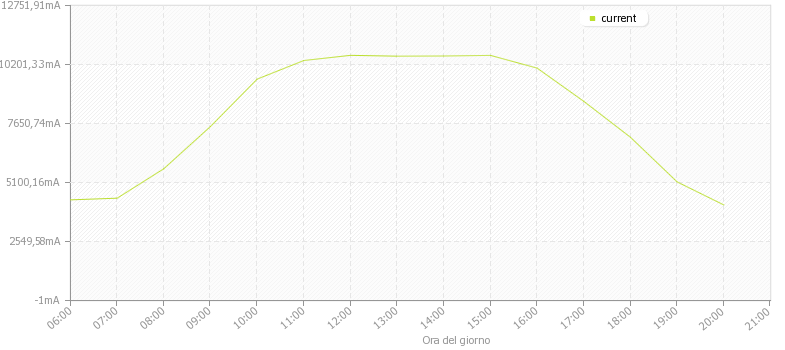
\includegraphics[width=400pt]{img/portale/corrente-stringa-giornaliera.png}
\end{figure}

\begin{figure}[!h]
\centering
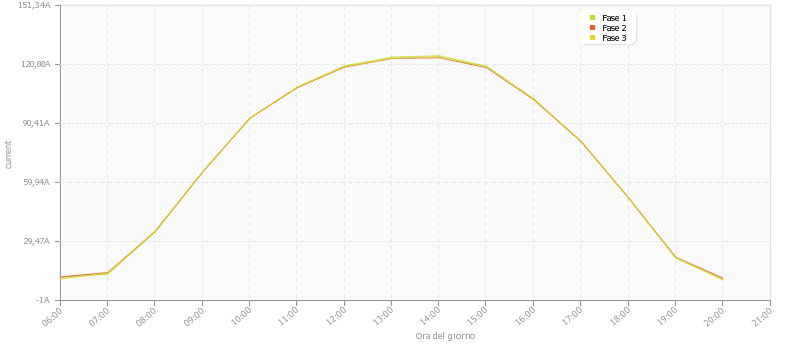
\includegraphics[width=400pt]{img/portale/current-power-transponder.png}
\end{figure}

\begin{figure}[!h]
\centering
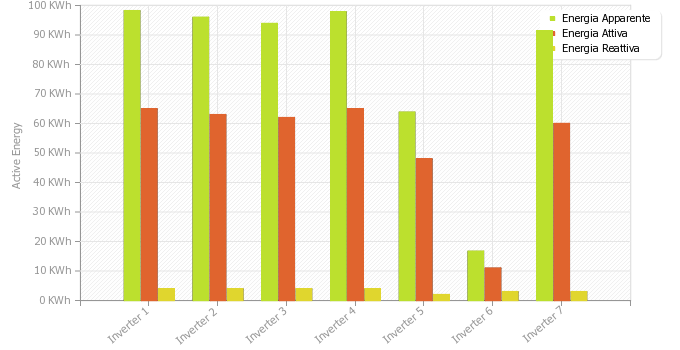
\includegraphics[width=400pt]{img/portale/energia-confronto-inverter.png}
\end{figure}



\begin{figure}[!h]
\centering
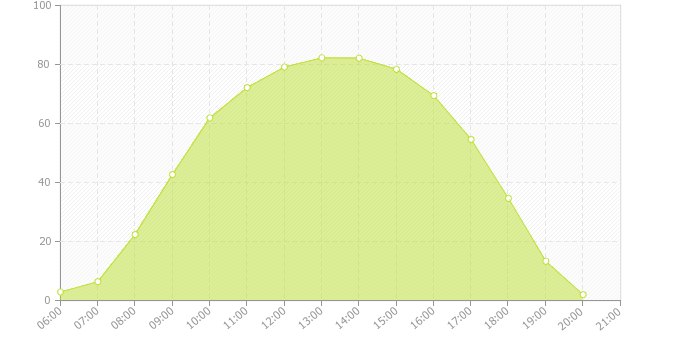
\includegraphics[width=400pt]{img/portale/potenza-giornaliera.png}
\end{figure}

\begin{figure}[!h]
\centering
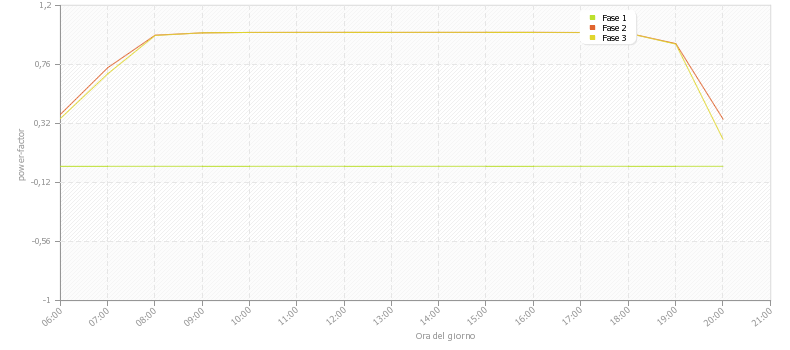
\includegraphics[width=400pt]{img/portale/power-factor-power-transponder.png}
\end{figure}



\begin{figure}[!h]
\centering
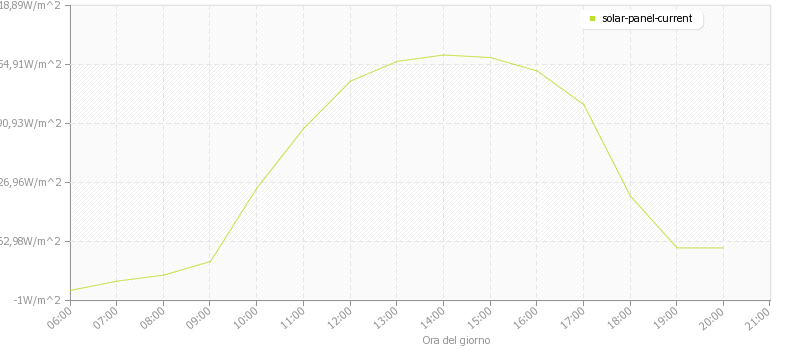
\includegraphics[width=400pt]{img/portale/radiazione-giornaliera.png}
\end{figure}
\begin{figure}[!h]
\centering
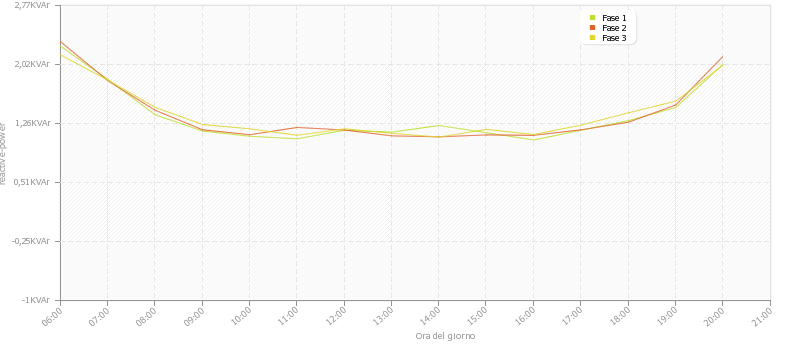
\includegraphics[width=400pt]{img/portale/reactive-power-power-transponder.png}
\end{figure}
\begin{figure}[!h]
\centering
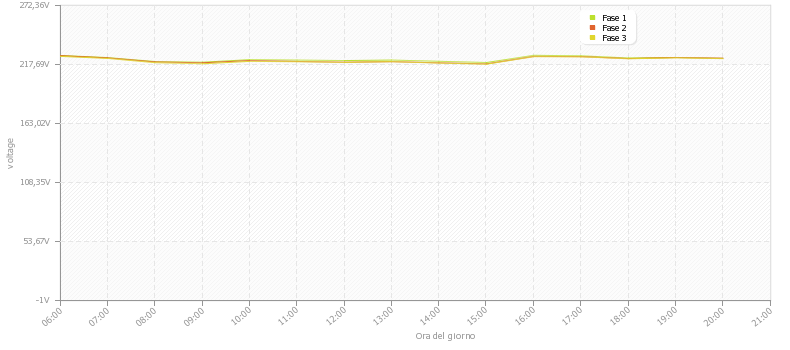
\includegraphics[width=400pt]{img/portale/voltage-power-transponder.png}
\end{figure}













